\part{Python programming I}
\section{Introduction}
\subsection*{General}
\begin{frame}[label=contents_prog1]
  \frametitle{Today's outline}
  \mode<beamer>{
    \only<1>{
      \begin{columns}
        \column{0.5\textwidth}
          \tableofcontents[sections={1-3}]
        \column{0.5\textwidth}
          \tableofcontents[sections={4-8}]
      \end{columns}}
  }
  \only<2>{
    \begin{columns}
      \column{0.5\textwidth}
        \tableofcontents[sections={1-3},currentsection]
      \column{0.5\textwidth}
        \tableofcontents[sections={4-8},currentsection]
    \end{columns}
    }
\end{frame}

\subsection{General programming}
\begin{frame}
  \frametitle{Why should you learn something about programming?}
  \begin{itemize}[<+->]
    \item Scientific analyses depend more than ever on computer programs and simulation methods
    \item Knowledge of programming allows you to automate routine tasks 
    \item Ability to understand algorithms by inspection of the code 
    \item Learn to think by dissecting a problem into smaller, easier to solve, parts 
  \end{itemize}\vskip2em
  \begin{columns}
    \column<1->{0.23\textwidth}
    \tikz\node[circle,draw,very thick,maincolor,
    text=white,minimum size=\columnwidth,
    path picture={
    \node at (path picture bounding box.center){
      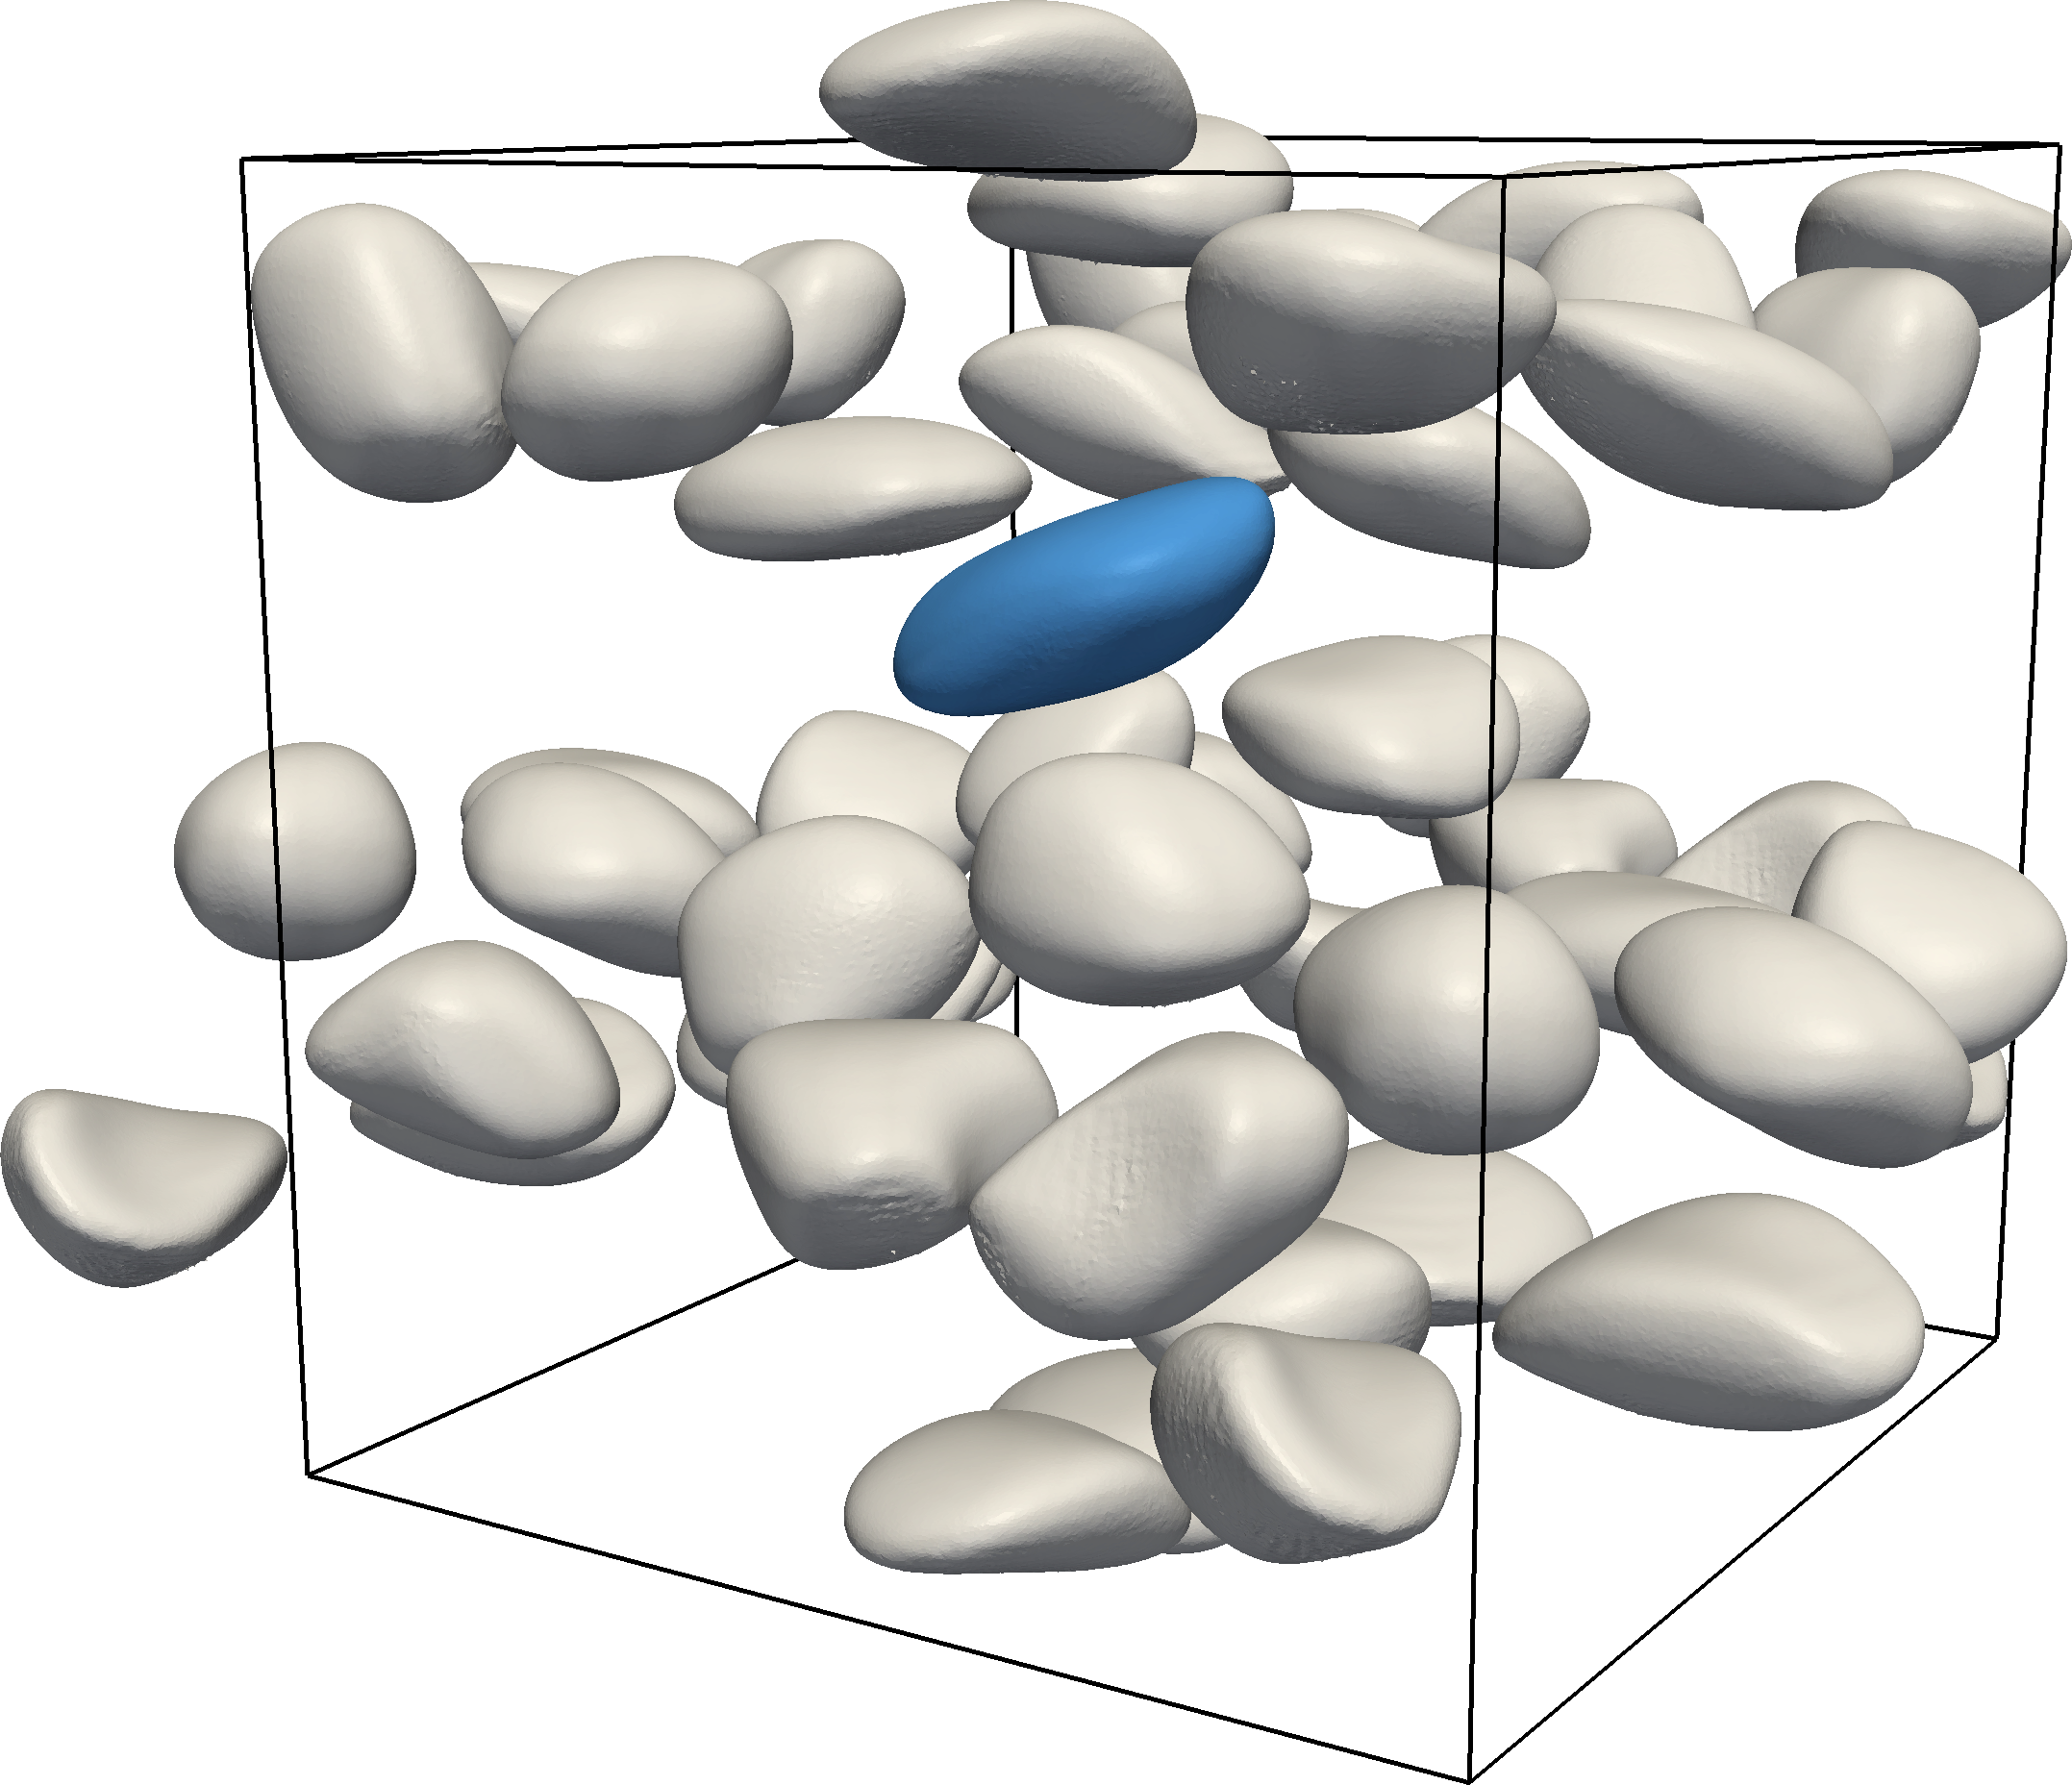
\includegraphics[width=\columnwidth]{sim1.png}
      };
      }]{};
  \column<2->{0.23\textwidth}
  \tikz\node[circle,draw,very thick,maincolor,
  text=white,minimum size=\columnwidth,
  path picture={
    \node at (path picture bounding box.center){
                   
\includegraphics[width=1.1\columnwidth]{automate.jpg}
                   };
                   }]{};
                   \column<3->{0.23\textwidth}
                   \tikz\node[circle,draw,very thick,maincolor,
                   text=white,minimum size=\columnwidth,
                   path picture={
               \node at (path picture bounding box.center){
                 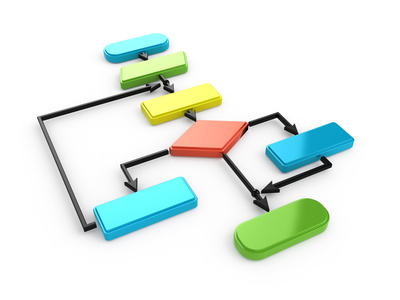
\includegraphics[width=1.2\columnwidth]{algorithm.jpg}
                 };
                 }]{};
                 \column<4>{0.23\textwidth}
                 \tikz\node[circle,draw,very thick,maincolor,
                 text=white,minimum size=\columnwidth,
                 path picture={
                   \node at (path picture bounding box.center){
                     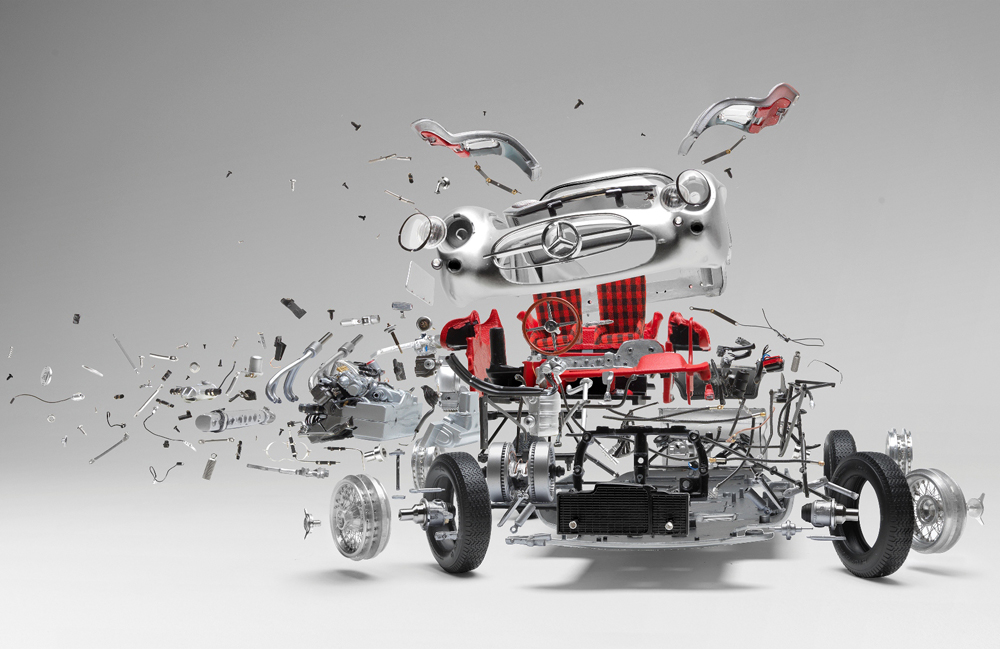
\includegraphics[width=1.5\columnwidth]{dissect.jpg}
                     };
                     }]{};
                    \end{columns}
                  \end{frame}
                  
                  \begin{frame}
                \frametitle{Introduction to programming}
                \begin{block}{What is a program?}
                  \emph{A program is a sequence of instructions that is written to perform a certain task on a computer.} % SOURCE http://www.greenteapress.com/thinkpython/html/thinkpython002.html
                \end{block}
                \begin{itemize}
                  \item The computation might be something mathematical, a symbolic operation, image analysis, etc.%such as solving a system of equations or finding the roots of a polynomial
                  % \item It can also be a symbolic computation, such as searching and replacing text in a document 
                  % \item A program may even be used to compile another program
                  % \item A program consists of one or more \emph{algorithms}
                \end{itemize}
                \begin{block}{Program layout}
  \begin{enumerate}
    \item Input (Get the radius of a circle)
    \item Operations (Compute and store the area of the circle)
    \item Output (Print the area to the screen)
  \end{enumerate}
\end{block}
\end{frame}

\begin{frame}
  \frametitle{Versatility of Python}
  \centering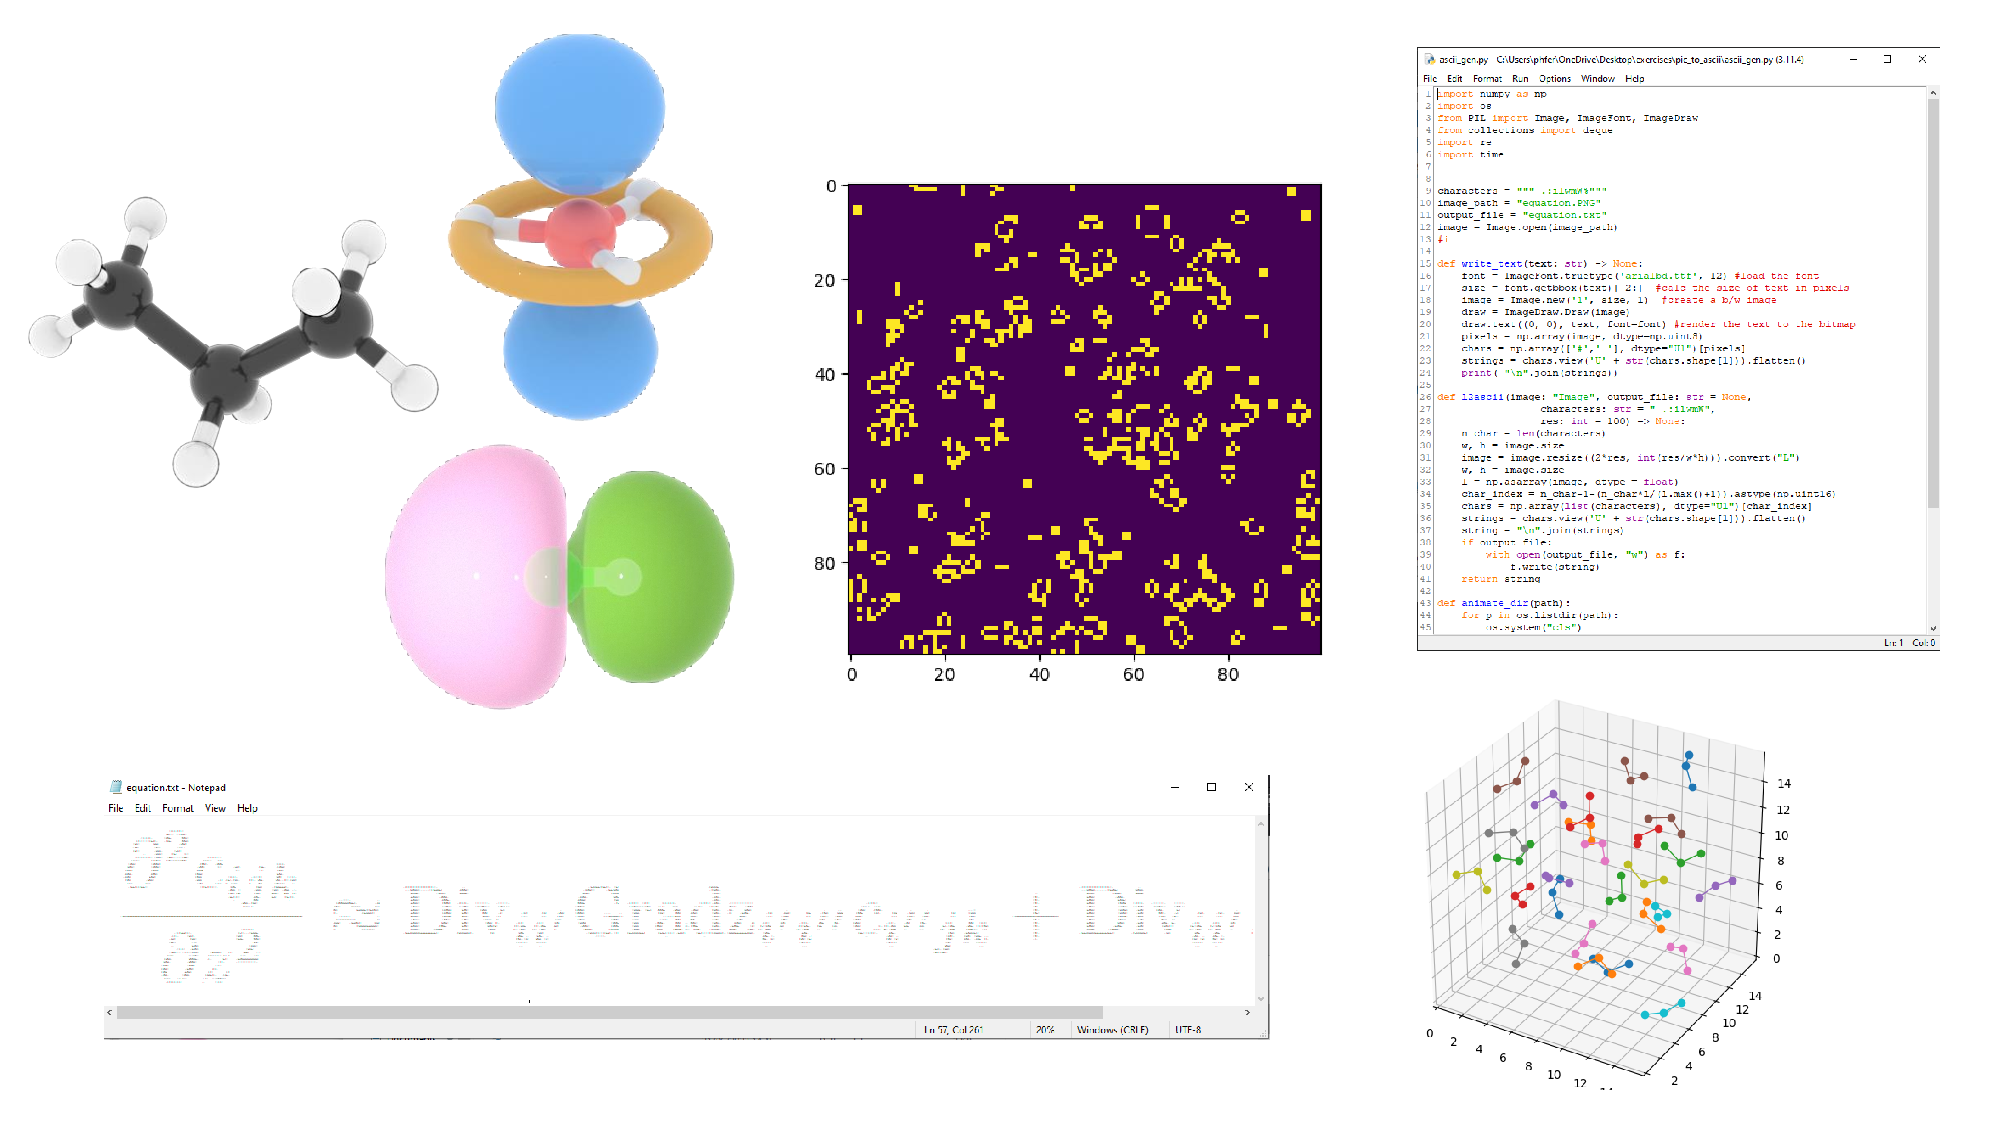
\includegraphics[width=0.9\textwidth]{python_versatility.pdf}
\end{frame}

\begin{frame}
  \frametitle{Versatility of Python: ODE solver}
  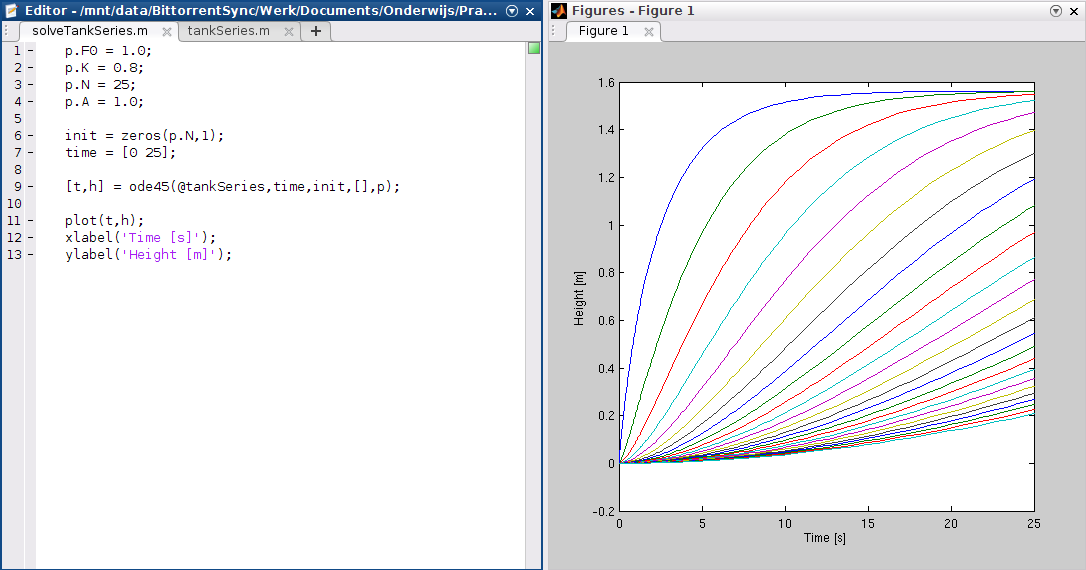
\includegraphics[width=\textwidth]{odesol.png}
\end{frame}

\begin{frame}[fragile]
  \frametitle{Versatility of Python: Image analysis}
  \vskip1em
  \begin{columns}[T]
    \column{0.5\textwidth}
    \begin{lstlisting}
# Importing necessary libraries
import numpy as np
from scipy import ndimage
from PIL.Image import fromarray
from skimage import io, color, feature, measure

# Loading and processing image 
I = io.imread('bub0.png')
BW = color.rgb2gray(I)
E = feature.canny(BW) 
F = ndimage.binary_fill_holes(E)

# Show final image
fromarray(F).show()
    \end{lstlisting}  
    \column{0.5\textwidth}
    \vfill
    \includegraphics<1>[width=\columnwidth]{bub1.png}
    \includegraphics<2>[width=\columnwidth]{bub2.png}
    \includegraphics<3>[width=\columnwidth]{bub3.png}
    \includegraphics<4>[width=\columnwidth]{bub4.png}
  \end{columns}
\end{frame}

{\nologo
\begin{frame}
  \frametitle{Versatility of Python: Curve fitting}
  \centering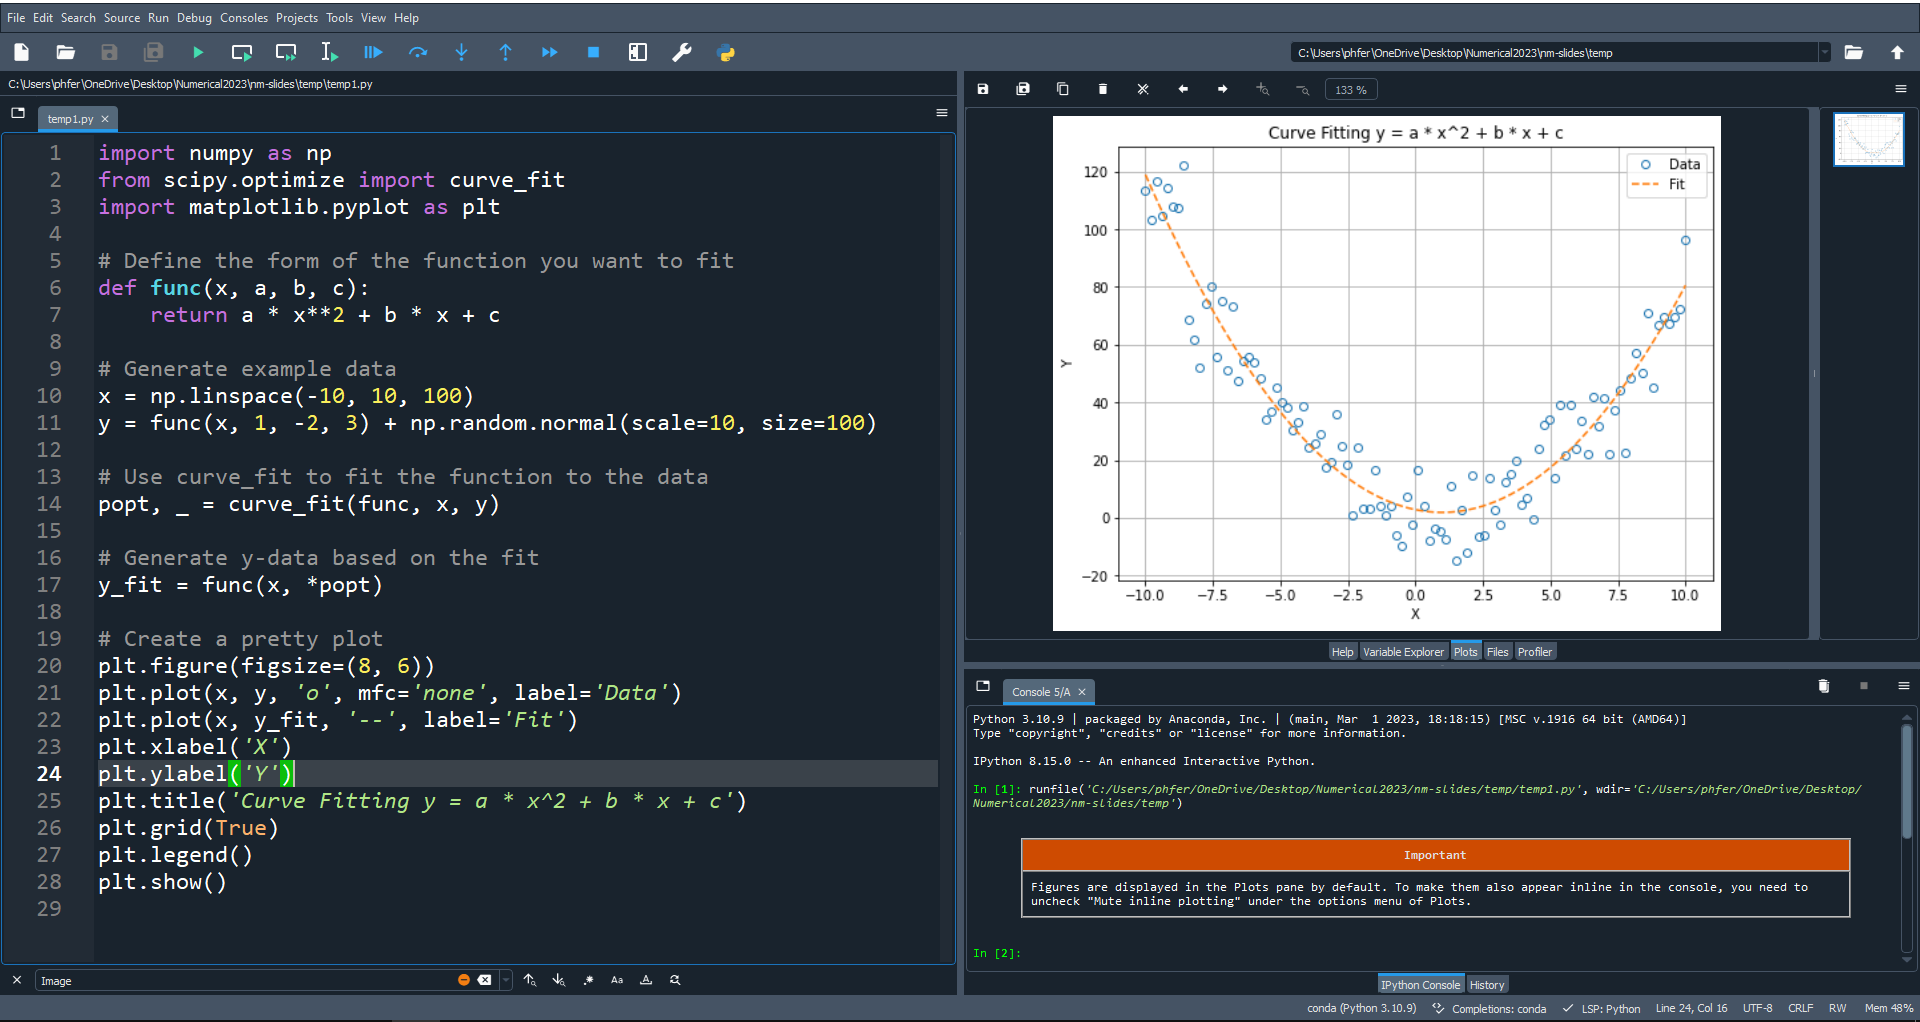
\includegraphics[width=\textwidth]{cftool.png}
\end{frame}
}

\subsection{First steps}
\begin{frame}[fragile]
  \frametitle{Getting started}
  \begin{itemize}
    \item Start the Python REPL (read–eval–print loop) by running \lstinline|python| or \lstinline|ipython|
    \item Enter the following commands on the command line. Evaluate the output.
  \end{itemize}
  \pause
  \begin{columns}
    \column{0.75\textwidth} 
      \begin{lstlisting}[numbers=none]
>>> 2 + 3        # Some simple calculations
>>> 2 * 3
>>> 2 * 3**2     # Powers are done using ** (*@ \pause @*)
>>> a = 2        # Storing values into the workspace
>>> b = 3
>>> c = (2 * 3)**2  # Parentheses set priority
>>> 10_000_000 / b (*@ \pause @*)
>>> print(a)
>>> print(a,b)
>>> print(a,b,c,sep='--')
>>> print("Numerical methods")
      \end{lstlisting}\pause
    \column{0.25\textwidth} 
      \begin{lstlisting}[style=PyOutput,numbers=none]
5
6
18



3333333.3333333335
2
2, 3
2--3--36
Numerical methods
      \end{lstlisting}
  \end{columns}
\end{frame}

\begin{frame}[fragile]
  \frametitle{Printing and formatting results}
  You can control the formatting of variables in string literals using various methods - we recommend f-strings. Note that formatting only changes how numbers are \emph{displayed}, not the underlying representation.

  \begin{lstlisting}[language=Python,numbers=none]
>>> a = 19/4
>>> print("Few digits {:.2f}".format(a)) # 2 decimal places
>>> print("Many digits {:.10f}".format(a)) # 10 decimal places
>>> 
>>> b = 22/7
>>> i = 13
>>> print("Almost pi: %1.4f" % b)
>>> print("i = %d, a = %1.4f and b = %1.8f" % (i,a,b))
>>>
>>> # Using f-strings (Python 3.6+)
>>> c = (21)**0.5 # sqrt of 21
>>> print(f"{c:.10f}") # Float with 10 decimal places
>>> mystr = f"{c:.2e}" # Scientific notation with 2 decimal places in a string object
>>> print(mystr) # Print the string object
>>> print(f"{b=}") # Use = to print variable name and value
>>> print(f"{b=:_^15.2}") # Adjust spacing and spacer character
  \end{lstlisting}
\end{frame}
 
 {\nologo
 \begin{frame}[fragile]
  \frametitle{A few helpful things}
  \begin{itemize}[<+->]
    \item Using the \keystroke{$\uparrow$} and \keystroke{$\downarrow$} keys, you can cycle through recent commands
    \item Typing part of a command and pressing \keystroke{Tab} completes the command and lists the possibilities
    \item If a computation takes too long, you can press \keystroke{Ctrl}+\keystroke{C} to stop the program and return to the command line. Stored variables may contain incomplete results.
    \item Sequences of commands (programs, scripts) are contained as py-files, plain text files with the \lstinline$.py$ extension.
    \item Python scripts (and notes/markdown) can also be contained in jupyter notebooks, which have extension \lstinline$.ipynb$.
    \item Such py-files must be in the \emph{current working directory} or in the Python \emph{path}, the locations where Python searches for a command. If you try to run a script that is not in the path, Python will throw an Exception/Error.
    \item Anything following a \lstinline$#$ symbol is regarded as a comment
    \item There are several keyboard shortcuts (vary with text editor) that will make coding much more efficient.
  \end{itemize}
\end{frame}
}

\begin{frame}[fragile]
  \frametitle{Scripts, notebooks and REPL}
  \begin{itemize}
    \item The REPL, indicated by the \lstinline|>>>| prompt, has the advantage of immediate result after typing a command.
    \item Larger programs are better written in separate files; either Jupyter notebooks (.ipynb files) or plain script files (.py files).
    \item Defining functions in such files will put them in the \emph{scope}, but will not run them until they are actually called.
    \item The snippets in these slides will continue to use the REPL for single-line commands, and move towards scripts when larger functions are being constructed.
  \end{itemize}
\end{frame}

\subsection{Further reading}
\begin{frame}[fragile]
\frametitle{Python help, documentation, resources}
\begin{itemize}
  \item Refer to the Python documentation at \href{https://docs.python.org/3/}{Official documentation}.
  \begin{itemize}
    \item Try for instance: \lstinline$help(print)$ or \lstinline$help(help)$.
  \end{itemize}
  \item Other packages that we will use:
  \begin{itemize}
    \item \href{https://numpy.org/doc/stable/}{NumPy documentation}
    \item \href{https://matplotlib.org/stable/}{Matplotlib documentation}
    \item \href{https://docs.scipy.org/}{SciPy documentation}
  \end{itemize}
  \item We supply a number of basic practice/reference modules: Python Crash Course.
  \item \href{https://tue.on.worldcat.org/oclc/1346554335}{Python Crash Course, 3rd Edition \faExternalLink} by Eric Matthes
  \item \href{https://tue.on.worldcat.org/oclc/1023864062}{A Whirlwind Tour of Python \faExternalLink} by Jake Vanderplas
  \item \href{https://tue.on.worldcat.org/oclc/1164494156}{Introduction to Scientific Programming with Python \faExternalLink} by Joakim Sundnes
  \item \href{https://pythonnumericalmethods.berkeley.edu/notebooks/Index.html}{Python Programming And Numerical Methods: A Guide For Engineers And Scientists \faExternalLink} by Kong, Siauw and Bayen
  \item Search the web, Reddit, YouTube, etc.
\end{itemize}
\end{frame}

\section{Data structures}
\subsection{Data types}
\againframe<2>{contents_prog1}
\begin{frame}[fragile]
 \frametitle{Terminology}
 \begin{description}
  \item[Variable] Piece of data stored in the computer memory, to be referenced and/or manipulated
  \item[Function] Piece of code that performs a certain operation/sequence of operations on given input
  \item[Operators] Mathematical operators (e.g. \lstinline$ + - *$ or \lstinline$/$), relational (e.g. \lstinline$< >$or \lstinline$==$, and logical operators (\lstinline$and$, \lstinline$or$)
  \item[Script] Piece of code that performs a certain sequence of operations without specified input/output
  \item[Expression] A command that combines variables, functions, operators and/or values to produce a result.
 \end{description}
\end{frame}

\begin{frame}[fragile]
 \frametitle{Variables in Python}
  \begin{itemize}
    \item Python stores variables in the \emph{namespace}
    \item You should recognize the difference between the \emph{identifier} of a variable (its name, e.g. \lstinline$x$, \lstinline$setpoint_p$), and the data that it actually stores (e.g. 0.5)
    \item Python also defines a number of functions by default, e.g. \lstinline$min$, \lstinline$max$ or \lstinline$sum$.
    \begin{itemize}
      \item A list of built-in methods is given by \lstinline$dir(__builtins__)$
    \end{itemize}
    \item You can assign a variable by the \lstinline$=$ sign:
   \begin{lstlisting}[language=Python, numbers=none]
>>> x = 4*3
>>> x
12
   \end{lstlisting}
   \item If you don't assign a variable, it will be stored in \lstinline$_$
   \item In most text editors, all variables are cleared automatically before the next execution. 
 \end{itemize}
\end{frame}

\begin{frame}[fragile]
  \frametitle{Datatypes and variables}
  Python uses different types of variables:
      \begin{longtable}{l!{\vrule}l}
       Datatype        & Example \\ \hline
       \lstinline$str$    & \lstinline$'Wednesday'$ \\
       \lstinline$int$    & \lstinline$15$ \\
       \lstinline$float$  & \lstinline$0.15$ \\
       \lstinline$list$   & \lstinline$[0.0, 0.1, 0.2, 'Hello', ['Another','List']]$ \\
       \lstinline$dict$   & \lstinline${'name': 'word', "n": 2}$ \\
       \lstinline$bool$   & \lstinline$False$ \\
       \lstinline$tuple$  & \lstinline$(True, False)$ \\
     \end{longtable}
     \pause
     Everything in Python is an object. You can use the \lstinline$dir()$ function to query the possible methods on an object of a datatype (e.g. \lstinline$(dir(list))$, \lstinline$dir(28)$ or \lstinline$dir("Yes!")$).
 \end{frame}

 %% LISTS SECTION
\subsection{Lists}
\begin{frame}[fragile]
  \frametitle{Lists in Python (1)}
  \begin{itemize}
    \item Lists are containers of collections of objects
    \item A list is initialized using square brackets with comma-separated elements
    \begin{lstlisting}[language=Python,numbers=none]
>>> brands = ['Audi', 'Toyota', 'Honda', 'Ford', 'Tesla']
    \end{lstlisting}
    \item Lists can contain and mix any object type, even other lists:
    \begin{lstlisting}[language=Python,numbers=none]
>>> another_list = [0.0, 0.1, 0.2, 'Hello', brands]
>>> print(another_list)
    \end{lstlisting}
    \begin{lstlisting}[style=PyOutput]
[0.0, 0.1, 0.2, 'Hello', ['Audi', 'Toyota', 'Honda', 'Ford', 'Tesla']]
    \end{lstlisting}
    \item Access (i.e., read) an entry in a list. Note that indexing starts at 0:
    \begin{lstlisting}[language=Python,numbers=none]
>>> print(another_list[0],another_list[3])
    \end{lstlisting}
    \begin{lstlisting}[style=PyOutput]
0.0 Hello
    \end{lstlisting}
  \end{itemize}
 \end{frame}
 
 \begin{frame}[fragile]
   \frametitle{Lists in Python (2)}
   \begin{itemize}
    \item Manipulate the value of an entry goes likewise:
    \begin{lstlisting}[language=Python,numbers=none]
>>> another_list[3] = 'Bye' # Becomes: [0.0, 0.1, 0.2, 'Bye', ['Audi', ...]]
    \end{lstlisting}
    \item Slicing is used to retrieve multiple elements:
    \begin{lstlisting}[language=Python,numbers=none]
>>> another_list[1:4] # This will give the elements from index 1 to index 3
    \end{lstlisting}
    \begin{lstlisting}[style=PyOutput]
[0.1, 0.2, 'Bye']
    \end{lstlisting}
    \item Lists can be unpacked into individual variables:
    \begin{lstlisting}[language=Python,numbers=none]
>>> a,b,c,d,e = brands
>>> print(f"The first list element was {a}, then {b}, {c}, {d} and finally {e}.")
    \end{lstlisting}
    \begin{lstlisting}[style=PyOutput]
The first list element was Audi, then Toyota, Honda, Ford and finally Tesla.
    \end{lstlisting}
    \item From here onwards, we will omit the \lstinline|print| statements from the slides
   \end{itemize}\vskip1em
  \end{frame}
 
  \begin{frame}[fragile]
    \frametitle{Lists in Python (3)}
    \begin{itemize}
      \item Lists can be concatenated or repeated by the addition and multiplication operators respectively: 
      \begin{lstlisting}[language=Python,numbers=none]
>>> more_brands = ['Nissan','Kia'] + brands
      \end{lstlisting}
      \begin{lstlisting}[style=PyOutput]
['Nissan', 'Kia', 'Audi', 'Toyota', 'Honda', 'Ford', 'Tesla']
      \end{lstlisting}
      \begin{lstlisting}[language=Python,numbers=none]
>>> zeros = 10*[0]
      \end{lstlisting}
      \begin{lstlisting}[style=PyOutput]
[0, 0, 0, 0, 0, 0, 0, 0, 0, 0]
      \end{lstlisting}
      \item Find out which methods can be performed on a list by using \lstinline|dir(more_brands)|:
      \begin{lstlisting}
more_brands.append('Volvo') # Append object (here: string literal) at the end of the list 
more_brands.insert(1,'BMW') # Insert object at index 1
more_brands.sort()          # Sorts the list in-place
item = more_brands.pop(3)   # Removes element at index 3 from the list, stores it as item
      \end{lstlisting}
    \end{itemize}
\end{frame}
 
 \begin{frame}[fragile]
   \frametitle{Lists in Python (4)}
   Ranges of numbers are set using the \lstinline|range(start=0,stop,step=1)| command:
   \begin{itemize}
    \item Create a list with a range of numbers:
    \begin{lstlisting}[language=Python,numbers=none]
>>> a = list(range(1, 11))     # Creates a list from 1 to 10
    \end{lstlisting}
    \item List comprehensions can be used to create lists with more complex patterns:
    \begin{lstlisting}[language=Python,numbers=none]
>>> x = [i/10 for i in range(-10, 11)]   # Creates a list from -1 to 1 with a step of 0.1
    \end{lstlisting}
    \item Manipulating multiple components using slicing and a loop:
    \begin{lstlisting}[language=Python,numbers=none]
>>> y = list(range(11))  # Creates a list from 0 to 10
>>> for i in [0, 3, 4, 5, 6]: 
>>>     y[i] = 1
    \end{lstlisting}
    \item Or (by supplying a list instead of a scalar):
    \begin{lstlisting}[language=Python,numbers=none]
>>> y[0:2] = [16, 19]  # Sets y[0] to 16 and y[1] to 19
    \end{lstlisting}
  \end{itemize}
 \end{frame}

\begin{frame}[fragile]
  \frametitle{Assignment of variables; value or reference}
  Consider the following code snippets:
  \begin{columns}[t]
    \column{0.4\textwidth}
    \begin{lstlisting}
>>> i = 3
>>> j = i 
>>> j = i + 3
>>> print(i,j)
>>> print(id(i), id(j)) # Print memory address of data
    \end{lstlisting}\pause
    \begin{lstlisting}[style=PyOutput]
3, 6
8885416 8885544
    \end{lstlisting}\pause
    \column{0.5\textwidth}
    \begin{lstlisting}
>>> list_a = ['aa', 1, 'bb', 12, True, 1.618]
>>> list_b = list_a
>>> list_b[2] = 'cc'
>>> print(list_a, list_b, sep='\n')
>>> print(id(list_a), id(list_b))
    \end{lstlisting}\pause
    \begin{lstlisting}[style=PyOutput]
['aa', 1, 'cc', 12, True, 1.618]
['aa', 1, 'cc', 12, True, 1.618]
140285003056512 140285003056512
    \end{lstlisting}\pause
  \end{columns}
  \begin{itemize}
    \item Primitive or immutable data types (e.g. \lstinline|int|, \lstinline|float|, \lstinline|str|, \lstinline|tuple|) are \emph{assigned by value}; the value is copied and changes do not affect the original variables.
    \item Mutable data types (e.g. \lstinline|list|, \lstinline|set|, \lstinline|dict|) are \emph{assigned by reference}; they are two names pointing to the same data, changing one affects the values of the other.
  \end{itemize}
\end{frame}


\begin{frame}[fragile,label=practice_lists]
  \frametitle{Practice}
  Given a vector 
  \[ 
     x = \left[2 \ 4 \ 6 \ 8 \ 10 \ 12 \ 14 \ 16 \ 18 \ 20 \ 30 \ 40 \ 50 \ 60 \ 70 \ 80 \right]
  \]
  \begin{itemize}
   \item Define the vector using \lstinline|range|'s, without typing all individual elements
   \pause
   \begin{onlyenv}<beamer> 
    \begin{lstlisting}[]
>>> x = list(range(2,20,2)) + list(range(20,90,10))
     \end{lstlisting}
     \pause
    \end{onlyenv}
   \item Investigate the meaning of the following commands:
   \begin{lstlisting}[language=Python, numbers=none]
>>> x[2]            
>>> x[0:5]          
>>> x[:-1]          
>>> y = x[4:]       
>>> y[3]            
>>> y.pop(3)      
>>> sum(x)    
>>> max(x)       
>>> min(x) 
>>> x[::-1]       
     \end{lstlisting}    
  \end{itemize}
 \end{frame}

%% STRING SECTION
\subsection{Strings}
\begin{frame}[fragile]
  \frametitle{Strings in Python (1)}
  Creating a string:
  \begin{lstlisting}[language=Python,numbers=none]
>>> s = "Hello, world!"
>>> len(s)
13
  \end{lstlisting}
  Accessing a character in a string:
  \begin{lstlisting}[language=Python,numbers=none]
>>> s[7]
'w'
  \end{lstlisting}
  Getting a substring:
  \begin{lstlisting}[language=Python,numbers=none]
>>> s[7:12]
'world'
  \end{lstlisting}
  Or separate by whitespace using a string method (see \lstinline|dir(s)|):
  \begin{lstlisting}[language=Python,numbers=none]
>>> s.split()
['Hello,', 'world!']
  \end{lstlisting}
\end{frame}

\begin{frame}[fragile]
  \frametitle{Strings in Python (2)}
  Replacing a substring with another string:
  \begin{lstlisting}[language=Python,numbers=none]
>>> s.replace('world', 'Python')
'Hello, Python!'
  \end{lstlisting}
  Converting to upper and lower case:
  \begin{lstlisting}[language=Python,numbers=none]
>>> s.upper()
'HELLO, WORLD!'
>>> s.lower()
'hello, world!'
  \end{lstlisting}
  You can combine methods with string literals too:
  \begin{lstlisting}[language=Python,numbers=none]
>>> s.replace('WoRlD'.lower(), 'Python')
'Hello, Python!'
>>> s.startswith('hello'.title())
True
  \end{lstlisting}
  Finding the starting index of a substring:
  \begin{lstlisting}[language=Python,numbers=none]
>>> s.index("world")
7
  \end{lstlisting}
\end{frame}

\begin{frame}[fragile,label=practice_strings]
  \frametitle{Practice}
  Given a string
  \begin{lstlisting}
>>> s = "Python programming is fun!"
  \end{lstlisting}
  \begin{itemize}
   \item Find and print the index of the word "is".
   \item Create a new string where "fun" is replaced with "awesome".
   \item Print the string in uppercase.
  \end{itemize}
  \begin{onlyenv}<beamer>
    \begin{lstlisting}[]
>>> s.index('is')
>>> p = s.replace('fun','awesome')
>>> print(p.upper())
    \end{lstlisting}
  \end{onlyenv}
 \end{frame}

 %% TUPLES SECTION
\subsection{Tuples}
\begin{frame}[fragile]
  \frametitle{Tuples in Python}
  A tuple is a built-in data type that contains an immutable sequence of values. 
  Creating a tuple:
  \begin{lstlisting}[language=Python,numbers=none]
>>> t = (1, 2, 3)
  \end{lstlisting}
  Accessing an element of a tuple:
  \begin{lstlisting}[language=Python,numbers=none]
>>> t[1]
2
  \end{lstlisting}
  Tuples are immutable, so we can't change their elements. However, we can create a new tuple based on the old one:
  \begin{lstlisting}[language=Python,numbers=none]
>>> t = t + (4, )
  \end{lstlisting}
  Finding the length of a tuple:
  \begin{lstlisting}[language=Python,numbers=none]
>>> len(t)
4
  \end{lstlisting}
\end{frame}

\begin{frame}[fragile,label=practice_tuples]
  \frametitle{Practice}
  Given a tuple
  \begin{lstlisting}
>>> t = (1, 2, 3, 4, 5, 6)
  \end{lstlisting}
  \begin{itemize}
   \item Access and print the third element of the tuple.
   \item Try to change the value of the second element of the tuple.
   \item Create a new tuple by concatenating a second tuple \((7, 8, 9)\) to the original tuple.
  \end{itemize}\pause
  \begin{onlyenv}<beamer>
    \begin{lstlisting}[]
t = (1, 2, 3, 4, 5, 6)
print(t[2])
t[2] = 6
t2 = t + (7,8,9)
print(t2)
    \end{lstlisting}
  \end{onlyenv}
 \end{frame}

%% DICTIONARY SECTION 
\subsection{Dictionaries}
\begin{frame}[fragile]
  \frametitle{Dictionaries in Python (1)}
  Creating a dictionary:
  \begin{lstlisting}[language=Python,numbers=none]
>>> d = {'a': 1, 'b': 2, 'c': 3}
  \end{lstlisting}
  Accessing a value by its key:
  \begin{lstlisting}[language=Python,numbers=none]
>>> d['b']
2
  \end{lstlisting}
  Modifying a value associated with a key:
  \begin{lstlisting}[language=Python,numbers=none]
>>> d['b'] = 47
  \end{lstlisting}
  Adding a new key-value pair:
  \begin{lstlisting}[language=Python,numbers=none]
>>> d['d'] = 4
  \end{lstlisting}
  Removing a key-value pair using pop:
  \begin{lstlisting}[language=Python,numbers=none]
>>> d.pop('d')
4
  \end{lstlisting}
\end{frame}

\begin{frame}[fragile]
  \frametitle{Dictionaries in Python (2)}
  Get all keys as a list:
  \begin{lstlisting}[language=Python,numbers=none]
>>> list(d.keys())
['a', 'b', 'c']
  \end{lstlisting}
  Get all values as a list:
  \begin{lstlisting}[language=Python,numbers=none]
>>> list(d.values())
[1, 47, 3]
  \end{lstlisting}
  Get all key-value pairs as a list of tuples:
  \begin{lstlisting}[language=Python,numbers=none]
>>> list(d.items())
[('a', 1), ('b', 47), ('c', 3)]
  \end{lstlisting}
\end{frame}

\begin{frame}[fragile,label=practice_dictionary]
  \frametitle{Practice}
  Given a dictionary
  \begin{lstlisting}[language=Python,numbers=none]
>>> d = { 'Alice': 24, 'Bob': 27, 'Charlie': 22, 'Dave': 30}
  \end{lstlisting}
  \begin{itemize}
   \item Access and print the age of 'Charlie'.
   \item Update 'Alice' age to 25.
   \item Add a new entry for 'Eve' with age 29.
   \item Print all the keys in the dictionary.
  \end{itemize}\pause
  \begin{onlyenv}<beamer>
    \begin{lstlisting}[]
>>> print(d['Charlie'])
>>> d['Alice'] = 25
>>> d['Eve'] = 29
>>> print(d.keys())
dict_keys(['Alice', 'Bob', 'Charlie', 'Dave', 'Eve'])
    \end{lstlisting}
  \end{onlyenv}
 \end{frame}

 \section{Control flow}
 \subsection{Loops}
 \againframe<2>{contents_prog1}
 
 %% Loops
\begin{frame}[fragile]
  \frametitle{Loops in Python (1)}
  The \lstinline$for$ loop is used to iterate over a sequence (e.g. lists, sets, tuples, dictionaries, strings). Any \emph{iterable} object can be listed over:
  \begin{lstlisting}[language=Python,numbers=none]
>>> for i in range(5):
...     print(i)
0
1
2
3
4
  \end{lstlisting}\pause
  You can iterate over a list directly:
  \begin{lstlisting}[language=Python,numbers=none]
>>> my_list = [1, 2, 3, 4, 5]
>>> for num in my_list:
...     print(num)
1
2
3
4
5
  \end{lstlisting}
\end{frame}

\begin{frame}[fragile]
  \frametitle{Loops in Python (2)}
  The \lstinline|enumerate| keyword returns both the \emph{index} as well as the \emph{list element}:
  \begin{lstlisting}[language=Python,numbers=none]
>>> my_list = ['aa', 1, 'bb', 12, True, 1.618034, []]
>>> for idx,elm in enumerate(my_list):
...     print(f'Element {elm} of type {type(elm)} at index {idx}')
  \end{lstlisting}
  \pause
  \begin{lstlisting}[style=PyOutput]
Element aa of type <class 'str'> at index 0
Element 1 of type <class 'int'> at index 1
Element bb of type <class 'str'> at index 2
Element 12 of type <class 'int'> at index 3
Element True of type <class 'bool'> at index 4
Element 1.618034 of type <class 'float'> at index 5
Element [] of type <class 'list'> at index 6
  \end{lstlisting}
\end{frame}

\begin{frame}[fragile]
  \frametitle{Loops in Python (3)}
  The `while` loop keeps going as long as a condition is \lstinline{True}:
  \begin{lstlisting}[language=Python,numbers=none]
>>> i = 0
>>> while i < 3:
...     print(i)
...     i += 1
0
1
2
  \end{lstlisting}\pause
  Use \lstinline|break| to exit a loop prematurely, and \lstinline|continue| to skip to the next iteration:
  \begin{lstlisting}[language=Python,numbers=none]
>>> for i in range(5):
...     if i == 3:
...         break
...     print(i)
0
1
2
  \end{lstlisting}
\end{frame}

\begin{frame}[fragile,label=practice_for]
  \frametitle{Practice}
  Given a list
  \begin{lstlisting}[language=Python,numbers=none]
>>> my_list = [1, 3, 7, 8, 9] 
  \end{lstlisting}
 
 \begin{itemize}
  \item Use a for loop to print each element of the list.\pause
  \item Use a while loop to print the values at indices 0 to 4.\pause
  \item Use a loop to find and print the index of the number 7 in the list.
 \end{itemize}
 \begin{onlyenv}<beamer>
  \begin{columns}[T]
    \column{0.33\textwidth}
      \begin{lstlisting}[]
>>> for i in my_list:
...    print(i)
      \end{lstlisting}
    \column{0.33\textwidth}
      \begin{lstlisting}[]
>>> c = 0
>>> while (c<4):
...    print(f"{my_list[c]=}")
...    c += 1
      \end{lstlisting}
    \column{0.33\textwidth}
      \begin{lstlisting}[]
>>> c = 0
>>> while not my_list[c] == 7:
...    c += 1
>>> print(my_list[c])
      \end{lstlisting}      
  \end{columns}
 \end{onlyenv}
\end{frame}

%% CONTROL STATEMENTS
\subsection{Branching}
\begin{frame}[fragile]
  \frametitle{Conditional Statements in Python}
  The Boolean type \lstinline|bool| has only 2 possible values: \lstinline|True| or \lstinline|False| \\
  The \lstinline{if} statement is used to execute a block of code only if a condition is evaluated to \lstinline|True|:
  \begin{lstlisting}[language=Python, numbers=none, deletekeywords={is,not}]
>>> x = 5
>>> if x > 0:
...     print("x is positive")
x is positive
  \end{lstlisting}\pause
  Use \lstinline{elif} to specify additional conditions, and \lstinline{else} to define what to do if no conditions are met:
  \begin{lstlisting}[language=Python, numbers=none, deletekeywords={is,not}]
>>> if x > 10:
...     print("x is greater than 10")
... elif x == 10:
...     print("x is exactly 10")
... else:
...     print("x is less than 10")
x is less than 10
  \end{lstlisting}
\end{frame}

\begin{frame}[fragile]
  \frametitle{Nested conditionals}
  Nesting conditions allows for more complex conditionals:
  \begin{lstlisting}[language=Python, numbers=none, deletekeywords={is,not}]
>>> if x > 0:
...     if x % 2 == 0: # The modulo operator % yields the remainder of a division
...         print("x is positive and even")
...     else:
...         print("x is positive but odd")
... else:
...     print("x is non-positive")
x is positive but odd
  \end{lstlisting}\pause
  The \lstinline{in} keyword can be used to check membership in a sequence:
  \begin{lstlisting}[language=Python, numbers=none, deletekeywords={is,not}]
>>> my_list = [1, 2, 3, 4, 5]
>>> if 3 in my_list:
...     print("3 is a member of the list")
3 is a member of the list
  \end{lstlisting}
\end{frame}

\begin{frame}[fragile]
  \frametitle{Combined conditionals}
  \begin{block}{Leap year determination}
    To be a leap year, the year number must be divisible by four, except for end-of-century years, which must be divisible by 400.
  \end{block}\pause
  We can create combined conditions using \lstinline|not|, \lstinline|and| and \lstinline|or| to determine whether we have a leap year:
  \pause
  \begin{lstlisting}[language=Python, numbers=none]
>>> year = 2024
>>> if year % 4 == 0 and (not year % 100 == 0 or year % 400 == 0):
...    print(f"{year} is a leap year.")
... else:
...    print(f"{year} is not a leap year.")
  \end{lstlisting}
\end{frame}

\begin{frame}[fragile]
  \frametitle{Conditionals in list comprehensions}
  List comprehensions can be extended with conditionals too:
  \begin{lstlisting}[language=Python, numbers=none]
>>> x = [i for i in range(0,31) if i%3 == 0]
>>> print(x)
[0, 3, 6, 9, 12, 15, 18, 21, 24, 27, 30]
  \end{lstlisting}\pause
  \vskip1em
  Conditions are not restricted to modulo's. Here we select artists who have an 'r' or 'R' in their name:
  \begin{lstlisting}[language=Python, numbers=none]
artists = ["Adele", "Harry Styles", "Stef Ekkel", "Ed Sheeran", "Nicki Minaj", "Ariana Grande", "Robbie Williams"]

my_artists = [artist for artist in artists if artist.lower().count('r') > 0]
print(my_artists)
['Harry Styles', 'Ed Sheeran', 'Ariana Grande', 'Robbie Williams']
  \end{lstlisting}
  
\end{frame}

\begin{frame}[fragile,label=practice_conditions]
  \frametitle{Practice}
  Consider the list:
  \begin{lstlisting}[language=Python, numbers=none]
>>> my_list = [x**3 for x in range(1,25,2)] # Cubes of odd numbers
  \end{lstlisting}  \pause
  \begin{itemize}
  \item Use an \lstinline{if} statement to check if 125 is in \lstinline{my_list}, and print a message indicating the result.
  \item Write a statement that checks and prints whether \lstinline{my_list[3]} is divisible by 3, and if not, print the remainder.
  \item Use a list comprehension to create a list of all numbers in \lstinline|my_list| that are not divisible by 5.
 \end{itemize}\pause
 \begin{onlyenv}<beamer>
  \begin{columns}[T]
    \column{0.33\textwidth}
    \begin{lstlisting}[]
>>> if 125 in my_list:
...     print('The number 125 was found in my_list!')
    \end{lstlisting}
    \column{0.33\textwidth}
    \begin{lstlisting}[]
>>> if my_list[3] % 3 == 0:
...     print(f'{my_list[3]} is divisible by 3')
... else:
...     print(f'The remainder of {my_list[3]} and 3 is {my_list[3]%3}')
    \end{lstlisting}
    \column{0.33\textwidth}
    \begin{lstlisting}
>>> k = [n for n in my_list if not n % 5 == 0 ]
    \end{lstlisting}
  \end{columns}
\end{onlyenv}
\end{frame}

%% FUNCTIONS 
\section{Functions}
\subsection{Defining functions}
\againframe<2>{contents_prog1}

\begin{frame}[fragile]
  \frametitle{Functions in Python (1)}
  Functions are defined using the \lstinline{def} keyword followed by the function name and a list of parameters in parentheses. The function body starts after the colon:
  \begin{lstlisting}[language=Python, numbers=none]
>>> def greet(name):
...     print(f"Hello, {name}!")
  \end{lstlisting}\pause
  Call the function with the necessary arguments:
  \begin{lstlisting}[language=Python, numbers=none]
>>> greet("Alice")
Hello, Alice!
  \end{lstlisting}\pause
  Functions can return values using the \lstinline{return} keyword:
  \begin{lstlisting}[language=Python, numbers=none]
>>> def add(a, b):
...     return a + b
  \end{lstlisting}\pause
  Capture the return value in a variable, e.g. \lstinline|result|:
  \begin{lstlisting}[language=Python, numbers=none]
>>> result = add(2, 3)
>>> print(result)
5
  \end{lstlisting}
\end{frame}

\begin{frame}[fragile]
  \frametitle{Functions in Python (2)}
  Default argument values can be specified, making the argument optional:
  \begin{lstlisting}[language=Python, numbers=none]
>>> def greet(name, greeting="Hello"):
...     print(f"{greeting}, {name}!")
  \end{lstlisting}\pause
  Call the function with or without the optional argument:
  \begin{lstlisting}[language=Python, numbers=none]
>>> greet("Bob")
Hello, Bob!
>>> greet("Bob", "Buzz off")
Buzz off, Bob!
  \end{lstlisting}\pause
  Python supports functions with a variable number of arguments:
  \begin{lstlisting}[language=Python, numbers=none]
>>> def my_function(*args):
...     print(args)
  \end{lstlisting}\pause
  Call the function with a varying number of arguments:
  \begin{lstlisting}[language=Python, numbers=none]
>>> my_function(1, 2, 3, "Hello")
(1, 2, 3, "Hello")
  \end{lstlisting}
\end{frame}

\begin{frame}[fragile]
  \frametitle{Functions in Python (3)}
  Functions can also return multiple values (also >2)
  \begin{lstlisting}[language=Python, numbers=none]
>>> def statistics(numbers):
...     return max(numbers), min(numbers)
  \end{lstlisting}\pause
  Let's call the function with some list:
  \begin{lstlisting}[language=Python, numbers=none]
>>> numlist = [94,12,6,19,33,14,81,56,43,22]
>>> print(statistics(numlist))
(94, 6)
  \end{lstlisting}\pause
  Store the elements in separate variables:
  \begin{lstlisting}[language=Python, numbers=none]
>>> a,b = statistics(numlist)
>>> print(f'{a=}, {b=}')
a=94, b=6
  \end{lstlisting}
\end{frame}

{\nologo
\begin{frame}[fragile]
  \frametitle{Functions in Python (4)}
  \begin{itemize}
    \item Functions are very useful for \emph{abstraction}:
    \begin{itemize}
      \item You can compartmentalize and 'hide' complex pieces of code\
      \item Retain flexibility through arguments
      \item You can reuse often used pieces of code, limiting copy-paste of code
    \end{itemize}
    \item Extending functionality or fixing bugs is done in 1 place\pause
    \item \bfseries{Documentation is crucial!}\pause
  \end{itemize}
  \begin{lstlisting}[language=Python, numbers=none]
>>> def statistics(numbers):
...     """Return the maximum and minimum of a list of numbers
...        Function arguments:
...        numbers: list of numbers"""
...     return max(numbers), min(numbers)
  \end{lstlisting}\pause
  \begin{lstlisting}[language=Python, numbers=none]
>>> help(statistics)
  \end{lstlisting}
  \begin{lstlisting}[style=PyOutput,keywords={statistics},keywordstyle=\bfseries]
Help on function statistics in module __main__:

statistics(numbers)
Return the maximum and minimum of a list of numbers
Function arguments:
numbers: list of numbers
  \end{lstlisting}
\end{frame}
}

{\nologo
\begin{frame}[fragile]
  \frametitle{Passing arguments by value or reference?}
  Recall that certain Python variables are assigned by value, and others reference; the same goes for passing arguments \footnote{\href{https://k0nze.dev/posts/python-copy-reference-none/}{https://k0nze.dev/posts/python-copy-reference-none/}}:
  \begin{itemize}
    \item Primitive or immutable data types are \emph{passed by value}; the value is copied and changes made inside the function will not affect the values stored in the variables passed to the function.
    \item Mutable data types (e.g. list, set, dict) are passed to a function \emph{by reference}; changes that are made inside the function do affect the values outside of the function.
  \end{itemize}
  \begin{columns}[t]
    
    \column{0.4\textwidth}
    Consider the function:

    \begin{lstlisting}
def func(x, y):
    x = x - 1 # Subtract 1
    y.pop()   # Remove last item
    \end{lstlisting}\pause
    \column{0.6\textwidth}
    % We call the function using an immutable data type (\lstinline|int|) and a mutable data type (\lstinline|list|):
    \begin{lstlisting}
i = 1
l = ['a', 'b']

func(i, l)

print(i, l)
    \end{lstlisting}
    \begin{lstlisting}[style=PyOutput]
1, ['a']      
    \end{lstlisting}
  \end{columns}
\end{frame}
}


\begin{frame}[fragile,label=practice_functions1]
  \frametitle{Practice}
  \begin{columns}[t]
    \column{0.5\textwidth}
        Define a function that computes the factorial of a number, $n!$:
        \[
          n! = 1 \times 2 \times 3 \times \ldots \times (n-1) \times n
        \]
      \column{0.5\textwidth}
        Compute $\exp{(x)}$ using the Taylor series, iterate until the change is smaller than $1\cdot 10^{-6}$:
        \[
          \exp{(x)} = 1 + x + \frac{x^2}{2!} + \frac{x^3}{3!} + \ldots + \frac{x^n}{n!}
        \]
        \end{columns}
    \pause \vskip1em
    \begin{onlyenv}<beamer>
    \begin{columns}[t]
      \column{0.5\textwidth}
      \begin{lstlisting}[language=Python]
def factorial(n):
    """Compute the factorial of n"""
    x = 1
    for i in range(1,n+1):
        x *= i
    return x
      \end{lstlisting}
      \column{0.5\textwidth}
      \begin{lstlisting}[language=Python]
def exponential(x, eps=1.0e-6):
    """Compute exponential of x with accuracy eps (default: 1.0e-6)"""
    i = 0
    taylor_terms = [x**i/factorial(i)]
    
    while taylor_terms[-1] >= eps:
        i += 1
        taylor_terms.append(x**i/factorial(i))
    
    return sum(taylor_terms), i
      \end{lstlisting}
    \end{columns}
  \end{onlyenv}
 \end{frame}

\subsection{Recursion}
\begin{frame}[label=recursion,fragile]
 \frametitle{Advanced topic: Recursion}
 \begin{columns}[T]
   \column{0.5\textwidth}
   \begin{itemize}
    \item<1-> In order to understand recursion, one must first understand recursion
    \item<2-> A recursive function includes a call to itself (a function within a function)
    \begin{itemize}
      \item<3-> This could lead to infinite calls;
      \item<3-> A base case is required so that recursion is stopped;
      \item<3-> Base case does not call itself, simply returns.
    \end{itemize}
 \end{itemize}
   \column{0.5\textwidth}
   \includegraphics<3>[width=0.6\columnwidth]{scoobydoo.jpg}
 \end{columns}
\end{frame}

\againframe{recursion}

\begin{frame}[fragile]
 \frametitle{Recursion: example}
 \begin{lstlisting}[language=Python]
def mystery(a, b):
  if b == 1:
      # Base case
      return a
  else:
      # Recursive function call
      return a + mystery(a, b-1)
 \end{lstlisting}
\vskip1em \pause
\begin{itemize}
  \item What does this function do? \pause
  \item Can you spot the error? \pause
  \item How deep can you go? Which values of b don't work anymore?
\end{itemize}
\end{frame}

\begin{frame}[fragile,label=practice_functions2]
  \frametitle{Practice}
        Define a function that computes the factorial of a number, $n!$, using recursion:
        \[
          n! = 1 \times 2 \times 3 \times \ldots \times (n-1) \times n
        \]
    \pause \vskip1em
    \begin{onlyenv}<beamer>
      \begin{lstlisting}[language=Python]
def factorial(n):
    """Compute the factorial of n"""
    assert isinstance(n,int) and n >= 0, 'Use positive integers only'

    if n==1:
      return 1
    else:
      return n*factorial(n-1) 
      \end{lstlisting}
    \end{onlyenv}
\end{frame}

%% SCOPE
\subsection{Scope}
\begin{frame}[fragile]
  \frametitle{Scope of functions and variables in Python}

  In Python, the scope of a variable refers to the regions of a program where that variable is accessible. Understanding the scope of variables helps to avoid bugs and maintain a clean codebase. The scopes in Python are categorized as follows:

  \begin{description}
    \item[Local Scope] Variables defined inside a function are in the local scope of that function. They can only be accessed within that function.
    \item[Enclosing Scope] In the case of nested functions, a function will have access to the variables of the functions it is nested within.
    \item[Global Scope] Variables defined at the top-level of a script are global and can be accessed by all functions in the script, unless overridden within a function.
    \item[Built-in Scope] Python has a number of built-in identifiers that should not be used as variable names as they have special significance. Examples include \textit{print}, \textit{list}, \textit{dict}, etc.
  \end{description}

  % Python follows the LEGB rule for name resolution: Local, Enclosing, Global, Built-in.
\end{frame}

{\nologo
\begin{frame}[fragile]
  \frametitle{Examples Variable Scope}
  \begin{columns}[T]
    \column[T]{0.5\textwidth}
      \textbf{1. Local Scope}:
    \column[T]{0.5\textwidth}
      \begin{lstlisting}[language=Python]
def my_func():
local_var = 100  # Local scope
    print(local_var)
      \end{lstlisting}
  \end{columns}
  {\color{scharlaken}\noindent\rule{\textwidth}{0.4pt}}
  \begin{columns}    
  \column[T]{0.5\textwidth}
    \textbf{2. Enclosing Scope}:
  \column[T]{0.5\textwidth}
    \begin{lstlisting}[language=Python]
def outer_func():
    outer_var = 200  # Enclosing scope
          
    def inner_func():
        print(outer_var)
    
    inner_func()
    \end{lstlisting}
  \end{columns}
  {\color{scharlaken}\noindent\rule{\textwidth}{0.4pt}}
  \begin{columns}[T]
    \column[T]{0.5\textwidth}
    \textbf{3. Global Scope}:
    \column[T]{0.5\textwidth}
      \begin{lstlisting}[language=Python]
global_var = 300  # Global scope

def another_func():
    print(global_var)
      \end{lstlisting}
    \end{columns}
    {\color{scharlaken}\noindent\rule{\textwidth}{0.4pt}}
    \begin{columns}[T]
      \column[T]{0.5\textwidth}
        \textbf{4. Built-in Scope}:
      \column[T]{0.5\textwidth}
        \begin{lstlisting}[language=Python]
print(max, min, len, str, int, list)
        \end{lstlisting}
    \end{columns}
\end{frame}
}

\begin{frame}[fragile]
  \frametitle{Exercise Variable Scope}
  Investigate the behavior of the following nested functions and variables with the same name:
  \begin{lstlisting}[language=Python]
def outer_func():
    outer_var = 200

    def inner_func():
        outer_var = 500
        print(outer_var)

    inner_func()
  \end{lstlisting}
\end{frame}

% \begin{frame}[fragile]
%   \frametitle{Passing arguments by value or reference?}
%   Recall that certain Python variables are assigned by reference; the same goes for passing arguments\footnote{\href{k0nze.dev}{https://k0nze.dev/posts/python-copy-reference-none/}}:
%   \begin{itemize}
%     \item Primitive or immutable data types are \emph{passed by value}; the value is copied and changes made inside the function will not affect the values stored in the variables passed to the function.
%     \item Mutable data types (e.g. list, set, dict) are passed to a function \emph{by reference}; changes that are made inside the function do affect the values outside of the function.
%   \end{itemize}
%   Consider:
%   \begin{lstlisting}
% def func(x, y):
%     x = x - 1
%     y.pop()

% i = 1
% l = ['a', 'b']

% func(i, l)

% print(i, l)
%   \end{lstlisting}

%   \begin{lstlisting}[PyOutput]
% 1, ['a']      
%   \end{lstlisting}
% \end{frame}

\subsection{Lambda functions}
\begin{frame}[fragile]
  \frametitle{Lambda functions (1)}
  Consider the mathematical function \(f(x) = x^2+e^x\) defined as a Python function block:
  \begin{lstlisting}[language=Python]
def f(x):
    from math import exp
    return x**2 + np.exp(x)
  \end{lstlisting}
  Note:
  \begin{itemize}
    \item The function is defined using the \lstinline|def| keyword.
    \item The variables and \lstinline|exp| function used are defined \emph{locally}. They will not be available globally unless defined as such.
    \item The function is defined in a Python script, not in a separate file.
  \end{itemize}
\end{frame}

\begin{frame}[fragile]
  \frametitle{Lambda functions (2)}
  If you do not want to create a new function block, you can create an \emph{lambda function}:
  Lambda functions are small, anonymous functions that can be instantiated in a single line, or even as an argument to a function.
  \begin{lstlisting}[language=Python]
from math import exp
f = lambda x: x**2 + exp(x)
  \end{lstlisting}
  \pause
  \begin{itemize}
    \item \lstinline[language=Python]|f|: the name of the function
    \item \lstinline[language=Python]|lambda|: used to define the inline function
    \item \lstinline[language=Python]|x|: the input argument (can be multiple, comma separated)
    \item \lstinline|:|: colon indicating the function definition will start
    \item \lstinline[language=Python]|x**2 + exp(x)|: the actual function
  \end{itemize}\pause
  \begin{lstlisting}[language=Python]
xsqr_exp = [f(x) for x in range(5)]
print(xsqr_exp)
  \end{lstlisting}
  \begin{lstlisting}[language=Python]
[1.0, 3.718281828459045, 11.38905609893065, 29.085536923187668, 70.59815003314424]
  \end{lstlisting}
\end{frame}

%% Modules
\section{Modules}
\againframe<2>{contents_prog1}
\subsection{Using modules}
\begin{frame}[fragile]
  \frametitle{Using Modules in Python (1)}
  Modules are files containing Python code, used to organize functionalities and reuse code across projects. To use a module, it must first be imported using the \lstinline{import} keyword. Here, we import the entire \lstinline{math} module:
  \begin{lstlisting}[language=Python, numbers=none]
>>> import math
  \end{lstlisting}\pause
  Once imported, use the dot notation to access functions and variables defined in the module:
  \begin{lstlisting}[language=Python, numbers=none]
>>> math.sqrt(16)
4.0
  \end{lstlisting}\pause
  You can import specific attributes from a module using the \lstinline{from ... import ...} syntax:
  \begin{lstlisting}[language=Python, numbers=none]
>>> from math import sqrt
>>> sqrt(16)
4.0
  \end{lstlisting}
\end{frame}

\begin{frame}[fragile]
  \frametitle{Using Modules in Python (2)}
  Alias module names using the \lstinline{as} keyword to shorten module names and avoid naming conflicts:
  \begin{lstlisting}[language=Python, numbers=none]
>>> import numpy as np
  \end{lstlisting}\pause
  To view the list of all functions and variables in a module, use the \lstinline{dir()} function:
  \begin{lstlisting}[language=Python, numbers=none]
>>> import math
>>> dir(math)
  \end{lstlisting}\pause
  Get help on how to use a module or a function using the \lstinline{help()} function:
  \begin{lstlisting}[language=Python, numbers=none]
>>> help(math.sqrt)
  \end{lstlisting}
\end{frame}

\subsection{Math module}
\begin{frame}[fragile]
  \frametitle{The math module}
  Many mathematical operations and concepts are available in the \href{https://docs.python.org/3/library/math.html}{math module}:
  \begin{columns}
    \column{0.5\textwidth}
    \begin{lstlisting}[language=Python]
from math import pi,sin,sqrt,log10\
,exp,floor,ceil,factorial,inf,log
print(pi)
print(sin(0.2*pi))
print(sqrt(2))
print(log10(10_000))
print(exp(1))
print(log(exp(2)))
print(floor(2.57))
print(ceil(2.57))
print(floor(-2.57))
print(round(2.4))
print(round(4.5))
print(factorial(5))
print(f"1 divided by infinity equals {1/inf}")
    \end{lstlisting}\pause
    \column{0.5\textwidth}
    \begin{lstlisting}[style=PyOutput]
      

3.141592653589793
0.5877852522924731
1.4142135623730951
4.0
2.718281828459045
2.0
2
3
-3
2
4
120
1 divided by infinity equals 0.0
    \end{lstlisting}
  \end{columns}
\end{frame}

\begin{frame}[fragile,label=practice_math_module]
  \frametitle{Practice}
  Use the math module to compute $y=\sin(x)$ for 9 equidistant points $x\in \left[0,2\pi\right]$, including end-points.
    \begin{itemize}
      \item Use \emph{list comprehensions} to generate the lists \lstinline|x| and \lstinline|y|
    \end{itemize}\pause
    \begin{onlyenv}<beamer>
      \begin{columns}[T]
        \column{0.5\textwidth}
        \begin{lstlisting}[]
from math import pi,sin
x_values = [x/8*2*pi for x in range(9)]
y_values = [sin(x) for x in x_values]

for x,y in zip(x_values,y_values):
    print(f"{x: 10.4f},{y: 10.4f}")
        \end{lstlisting}\pause
      \column{0.5\textwidth}
      \begin{lstlisting}[style=PyOutput]
0.0000,    0.0000
0.7854,    0.7071
1.5708,    1.0000
2.3562,    0.7071
3.1416,    0.0000
3.9270,   -0.7071
4.7124,   -1.0000
5.4978,   -0.7071
6.2832,   -0.0000
      \end{lstlisting}
      \end{columns}
      
    \end{onlyenv}
\end{frame}


% \begin{frame}[fragile]
%   \frametitle{Practice}
%   \begin{columns}[T]
%     \begin{column}{0.5\textwidth}
%       \begin{enumerate}
%         \item Import the \lstinline{random} module and use a function from it to generate a random number.\pause
%         \begin{lstlisting}[language=Python]
% import random
% print(random.randint(1, 100))
%         \end{lstlisting}
%         The \lstinline{random.randint} function is used to generate a random integer number between 1 and 100. Alternatively, the \lstinline|random.random()| function generates a random float in the interval $[0,1)$.
%       \end{enumerate}
%     \end{column}

%     \begin{column}{0.5\textwidth}
%       \begin{enumerate}\setcounter{enumi}{1}
%         \item Import only the \lstinline{pi} variable from the \lstinline{math} module and print its value.\pause
%         \begin{lstlisting}[language=Python]
% from math import pi
% print(pi)
%         \end{lstlisting}
%         The \lstinline{pi} variable is imported from the \lstinline{math} module and its value is printed.
%         \item Create an alias for a module you import and use a function from the aliased module. \pause
%         \begin{lstlisting}[language=Python]
% import math as m
% print(m.sqrt(16))
%         \end{lstlisting}
%         The \lstinline{math} module is aliased as \lstinline{m} and the \lstinline{sqrt} function is used to find the square root of 16.
%       \end{enumerate}
%     \end{column}
%   \end{columns}
% \end{frame}

% \begin{frame}[fragile]
%   \frametitle{Practice}
%   \begin{columns}[T]
%     \begin{column}{0.5\textwidth}
%       \begin{enumerate}
%         \item Create a function that function to work on a range of numbers?
%         Remember list comprehensions
%         Compute y=sin(x)
%          for 8 equidistant points of x∈[0,2π]
%         \begin{lstlisting}[language=Python]
% import random
% print(random.randint(1, 100))
%         \end{lstlisting}
%         The \lstinline{random.randint} function is used to generate a random integer number between 1 and 100. Alternatively, the \lstinline|random.random()| function generates a random float in the interval $[0,1)$.
%       \end{enumerate}
%     \end{column}

%     \begin{column}{0.5\textwidth}
%       \begin{enumerate}\setcounter{enumi}{1}
%         \item Import only the \lstinline{pi} variable from the \lstinline{math} module and print its value.\pause
%         \begin{lstlisting}[language=Python]
% from math import pi
% print(pi)
%         \end{lstlisting}
%         The \lstinline{pi} variable is imported from the \lstinline{math} module and its value is printed.
%         \item Create an alias for a module you import and use a function from the aliased module. \pause
%         \begin{lstlisting}[language=Python]
% import math as m
% print(m.sqrt(16))
%         \end{lstlisting}
%         The \lstinline{math} module is aliased as \lstinline{m} and the \lstinline{sqrt} function is used to find the square root of 16.
%       \end{enumerate}
%     \end{column}
%   \end{columns}
% \end{frame}


\subsection{The random module}
\begin{frame}[fragile]
  \frametitle{The random module (1)}
  Random number generators and sampling tools are available through the \href{https://docs.python.org/3/library/random.html}{random module}. A few examples for \href{https://docs.python.org/3/library/random.html#functions-for-integers}{integers and sequences}:
  \begin{lstlisting}
import random as rnd

# Random integers
random_integers = [rnd.randint(0,10) for i in range(10)]
print(f'{random_integers = }')

# Sample from given population
my_range = range(12) # [0, 1, 2, ..., 11]
select_from_range = rnd.sample(my_range,8)
print(f'{select_from_range = }') # Selected 8 elements

# Choose 1 element from list
days_of_week = ['Monday','Tuesday','Wednesday','Thursday','Friday','Saturday','Sunday']
day = rnd.choice(days_of_week)
print(f"I've chosen {day} as my lucky day!")
  \end{lstlisting}\pause

  \begin{lstlisting}[style=PyOutput]
random_integers = [6, 6, 2, 5, 5, 8, 3, 7, 3, 4]
select_from_range = [2, 3, 10, 1, 6, 4, 8, 5]
I've chosen Wednesday as my lucky day!
  \end{lstlisting}
\end{frame}

\begin{frame}[fragile]
  \frametitle{The random module (2)}
  Examples for \href{https://docs.python.org/3/library/random.html#real-valued-distributions}{real valued distributions}:
  \begin{lstlisting}
import random as rnd

# Random number (uniform distribution) 0 < x < 1
x = [rnd.random() for i in range(5)]
print(x)

# Random number (uniform distribution) between given bounds
x = [rnd.uniform(1,3) for i in range(5)]
print(x)

# Random number from a Gauss distribution (mu=0, sigma=2)
x = [rnd.gauss(0,2) for i in range(5)]
print(x)
  \end{lstlisting}\pause

  \begin{lstlisting}[style=PyOutput,basicstyle=\tiny\ttfamily]
[0.6697878114597362, 0.4136014290205997, 0.5108247513505662, 0.44260043089156076, 0.9902269207988261]
[2.4749381508841077, 2.943448233960596, 2.516639180020423, 1.0481550073898795, 1.961356325508141]
[1.8199856149229392, 2.000097897306016, -2.4604868187736026, -0.46836605162997846, -2.5069012642608803]
  \end{lstlisting}
\end{frame}
  
\begin{frame}[fragile,label=practice_random]
  \frametitle{Practice}
  \begin{itemize}
    \item Create a \emph{function} that returns a list of $N$ dice throws (cubic dice, values 1-6)
    \item Throw the dice many times
    \item Print for each value how often it has been thrown
  \end{itemize} \pause
  \begin{onlyenv}<beamer>
    \begin{lstlisting}
import random as rnd

def throw_dice(N):
    return [rnd.randint(1,6) for _ in range(N)]

throws = throw_dice(40)
print(throws)

for i in range(1,7):
    n = len([t for t in throws if t==i])
    print(f"Value {i} was thrown {n} times")
        \end{lstlisting}\pause
  \end{onlyenv}
  \begin{lstlisting}[style=PyOutput,basicstyle=\tiny\ttfamily]
[5, 1, 1, 4, 6, 3, 3, 1, 5, 6, 1, 1, 1, 1, 5, 5, 2, 1, 1, 2, 2, 5, 5, 4, 6, 1, 3, 5, 6, 3, 1, 5, 6, 2, 3, 1, 6, 3, 2, 1]
Value 1 was thrown 13 times
Value 2 was thrown 5 times
Value 3 was thrown 6 times
Value 4 was thrown 2 times
Value 5 was thrown 8 times
Value 6 was thrown 6 times
  \end{lstlisting}
\end{frame}

 

% \begin{frame}[fragile]
%  \frametitle{Recursion: exercise}
%  Create a function computing the factorial of $N$, based on recursion. \pause
%  \begin{lstlisting}[language=Python]
% def fact_recursive(x):
%     # Catch non-integer and negative cases
%     if not isinstance(x, int) or x < 0:
%         print("You should provide a positive integer number only")
%         return None

%     # Recursive case
%     if x > 1:
%         return x * fact_recursive(x - 1)

%     # Base case
%     else:
%         return 1
%  \end{lstlisting}
% \end{frame}

\section{Conclusions}
\subsection*{Conclusions}
\againframe<2>{contents_prog1}
\begin{frame}[fragile]
  \frametitle{In conclusion...}
  \begin{itemize}
    \colorize<1> \item Python: A versatile development language. Easy to use libraries makes this language multi-purpose and easy to use.
    \colorize<2> \item Programming basics: variables, operators and functions, locality of variables, modules and recursive operations
  \end{itemize}
  \pause
    \begin{itemize}
    \colorize<3> \item For now: exercises on slide deck and Python modules
  \end{itemize}
\end{frame}

\section{Exercises}
\subsection*{Exercise 1}
\begin{frame}[fragile,label=practice_vectors_arrays]
  \frametitle{Practice vectors and arrays}
  \begin{enumerate}
    \item Create a list \lstinline|x| with the elements:
    \begin{itemize}
      \item \lstinline|[2, 4, 6, 8, ..., 16]|
      \item \lstinline|[0, 0.5, 2/3, 3/4, ..., 99/100]|
    \end{itemize}
    \item Create a list \lstinline|x| with the elements: \(x_n = \frac{(-1)^n}{2n-1}\) for \(n=1,2,3,\ldots,200\). Find the sum of the first 50 elements \(x_1,\ldots,x_{50}\).
    \item Let \lstinline|x = list(range(20, 201, 10))|. Create a list \lstinline|y| of the same length as \lstinline|x| such that:
    \begin{itemize}
      \item \lstinline|y[i] = x[i] - 3|
      \item \lstinline|y[i] = x[i]| for every even index \(i\) and \lstinline|y[i] = x[i] + 11| for every odd index \(i\).
    \end{itemize}
    \item Let \lstinline|T = np.array([[3, 4, 6], [1, 8, 6], [-4, 3, 6], [5, 6, 6]]).T|. Perform the following operations on T:
    \begin{itemize}
      \item Retrieve a list consisting of the 2nd and 4th elements of the 3rd row.
      \item Find the minimum of the 3rd column.
      \item Find the maximum of the 2nd row.
      \item Compute the sum of the 2nd column
      \item Compute the mean of the row 1 and the mean of row 3
    \end{itemize}
  \end{enumerate}
 \end{frame}


 \begin{frame}[fragile]
  \frametitle{Practice plotting}
  \begin{enumerate}
    \item Plot the functions $f(x)=x,\ g(x)=x^3,\ h(x)=e^x$ and $z(x)=e^{x^2}$ over the interval $[0,4]$ on the normal scale and on the log-log scale. Use an appropriate sampling to get smooth curves. Describe your plots by using the functions: \lstinline$plt.xlabel$, \lstinline$plt.ylabel$, \lstinline$plt.title$ and \lstinline$plt.legend$.
    \vskip1em
    \item Make a plot of the functions: $f(x)=sin(1/x)$ and $g(x)=cos(1/x)$ over the interval $[0.01,0.1]$. How do you create \lstinline$x$ so that the plots look sufficiently smooth?
  \end{enumerate}
 \end{frame}

 \begin{frame}[fragile]
  \frametitle{Practice control flow and loops (1)}
  \begin{enumerate}
    \item Write a function that uses two logical input arguments with the following behaviour:
    \begin{align*}
       f(\text{true},\text{true}) \mapsto \text{false} \\
      f(\text{false},\text{true}) \mapsto \text{true} \\ 
      f(\text{true},\text{false}) \mapsto \text{true} \\
      f(\text{false},\text{false}) \mapsto \text{false} \\
    \end{align*}
    \item Write a function that computes the factorial of x:
    \[ f(x) = x! = 1 \times 2 \times 3 \times 4 \times \ldots \times x \]
    \begin{itemize}
      \item Using a loop-construction
      \item Using recursion
    \end{itemize}
  \end{enumerate}
 \end{frame}

 \begin{frame}[fragile]
  \frametitle{Practice control flow and loops (2)}
  \begin{enumerate}
    \item Write a function that computes the exponential function using the Taylor series
    \[  e^x = 1 + x + \frac{x^2}{2!} + \frac{x^3}{3!} + \ldots \]
    until the last term is smaller than $10^{-6}$.
    \item Use a script to compute the result of the following series:
    \[
      f_n = \sum_{n=1}^{\infty} \frac{1}{\pi^2 n^2}
    \]
    This should give you an indication of the fraction this series converges to.
    \begin{itemize}
      \item Now plot in two vertically aligned subplots i) The result as a function of $n$, and ii) the difference with the earlier mentioned fraction as a function of n. For the latter, consider carefully the axis scale!
      % \item Use \lstinline$tic$ and \lstinline$toc$ to compare the computing times with $\pi^2$ inside vs outside the loop.
    \end{itemize}
  \end{enumerate}
 \end{frame}

 \begin{frame}[fragile]
  \frametitle{Practice logical indexing}
  \begin{enumerate}
    \item Let \lstinline$x = np.linspace(-4,4,1000)$, $y_1 = 3x^2 - 4x - 6$ and $y_2 = 1.5x - 1$. Use logical indexing to determine function $y_3 = \mathrm{max}(\mathrm{max}(y_1,y_2),0)$. Plot the function.
    \item Consider these data concerning the age (in years), length (in cm) and weight (in kg) of twelve adult men: \lstinline$A = [41 25 33 29 64 34 47 38 49 32 26 26]; H = [165 186 177 190 156 174 164 205 184 190 165 171]; W = [75 90 97 60 74 65 101 85 91 75 87 70];$.
    \begin{itemize}
      \item Calculate the average of all vectors (age, weight and length).
      \item Combine the command \lstinline$length$ with logical indexing to determine how many men in the group are taller than 182 cm.
      \item What is the average age of men with a body-mass index ($B \equiv \frac{W}{L^2}$ with $W$ in kg and $L$ in m) larger than 25? And for men with a $B<25$?
      \item How many men are older than the average and at the same time have a BMI below 25?
    \end{itemize}
  \end{enumerate}
 \end{frame}

\begin{frame}[fragile]
  \frametitle{Practice algorithm: Fourier series for heat equation}
  The unsteady 1D heat equation in 1D in a slab of material is given as:
  \[
     \frac{\partial T}{\partial t} = k\frac{\partial^2 T}{\partial x^2}
  \]
 We can express the temperature profile $T(x,t)$ in the slab using a Fourier sine series. For an initial profile T(x,0) = 20 and fixed boundary values T(0,t) = T(L,t) = 0, the solution is given as:
  \[
     T(x,t) = \sum_{n=1}^{n=\infty}\frac{40(1-(-1)^n)}{n\pi}  \sin\left(\frac{n\pi x}{L}\right) \exp\left(-kt\frac{n \pi}{L}^2\right)
  \]
  \begin{itemize}
      \item Create a script to solve this equation using loops and/or conditional statements
  \end{itemize}
 \end{frame}
 
%  \begin{frame}[fragile]
%   \frametitle{Fourier series for heat equation (1)}
%   A simple construct with a double loop.
%    \begin{lstlisting}
%  L = 2;
%  k = 0.004;
%  t = 3;
%  x = 0:0.1:L;
%  s = 0;
 
%  for n = 1:50
%      for i = 1:length(x)
%          pt(i) = 40*(1-(-1)^n)/(n*pi) * sin(n*pi*x(i)/L) * exp(-k*t*(n*pi/L)^2);
%      end
%      s = s + pt;
%  end
 
%  plot(x,s)
%    \end{lstlisting}
%  \end{frame}
 
%  \begin{frame}[fragile]
%   \frametitle{Fourier series for heat equation (2-1)}
%  We can also solve the equation for the entire x-range in 1 go. \lstinline$part$ and $s$ are both vectors. This is more efficient.
%    \begin{lstlisting}
%  L =  2;
%  x = linspace(0,L,101);
%  k = 0.004;
%  t = 3;
 
%  s = 0;
%  for n = 1:50
%      part = 40*(1-(-1)^n)/(n*pi) * sin(n*pi*x/L) * exp(-k*t*(n*pi/L)^2);
%      s = s + part;
%  end
 
%  plot(x,s)
%    \end{lstlisting}
%  \end{frame}
 
%  \begin{frame}[fragile]
%   \frametitle{Fourier series for heat equation (2-2)}
%  We can break the for-loop when the calculations are precise enough using an if-statement and a break-command.
%    \begin{lstlisting}
%  L = 2;
%  x = linspace(0,L,101);
%  k = 0.004;
%  t = 3;
 
%  s = 0;
%  for n = 1:2:50
%      part = 40*(1-(-1)^n)/(n*pi) * sin(n*pi*x/L) * exp(-k*t*(n*pi/L)^2);
%      s = s + part;
%      if (max(abs(part)) < 1e-6)
%          n
%          break
%      end
%  end
 
%  plot(x,s)
%    \end{lstlisting}
%  \end{frame}
 
%  \begin{frame}[fragile]
%   \frametitle{Fourier series for heat equation (3-1)}
%  We can run a while-loop for indeterminate iterations to ensure a certain precision while keeping computational demands to a minimum:
%    \begin{lstlisting}
%  L =  2;
%  x = linspace(0,2,101);
%  k = 0.004;
%  t = 3;
 
%  s = 0;
%  n = 1;
%  part = 1;
%  while (max(abs(part))>1e-6)
%      part = 40*(1-(-1)^n)/(n*pi) * sin(n*pi*x/L) * exp(-k*t*(n*pi/L)^2)
%      s = s + part;
%      n = n + 2;
%  end
 
%  n
%  plot(x,s)
%    \end{lstlisting}
%  \end{frame}
 
%  \begin{frame}[fragile]
%   \frametitle{Fourier series for heat equation (3-2)}
%  The \lstinline$drawnow$ command makes sure a plot is drawn before subsequent commands are executed. This gives us insight in the iteration process:
%    \begin{lstlisting}
%  L =  2;
%  x = linspace(0,2,101);
%  k = 0.004;
%  t = 3;
 
%  s = 0;
%  n = 1;
%  part = 1;
%  while (max(abs(part))>1e-6)
%      part = 40*(1-(-1)^n)/(n*pi) * sin(n*pi*x/L) * exp(-k*t*(n*pi/L)^2)
%      s = s + part;
%      n = n + 2;
%      plot(x,s)
%      pause(0.4)
%      drawnow
%  end
 
%  n
%    \end{lstlisting}
%  \end{frame}

%  \begin{frame}[fragile]
%   \frametitle{Fourier series for heat equation (as a function)}
%  A rudimentary function (i.e. no comments or checks) to get the heat equation profile for a given length, heat diffusivity and time:
%    \begin{lstlisting}
%  function [s,x] = fourier_series_heat_eqn(L,k,t)
%  x = linspace(0,L,101);
 
%  s = 0;
%  n = 1;
%  part = 1;
%  while (max(abs(part))>1e-6)
%      part = 40*(1-(-1)^n)/(n*pi) * sin(n*pi*x/L) * exp(-k*t*(n*pi/L)^2);
%      s = s + part;
%      n = n + 2;
%  end
%    \end{lstlisting}
   
%  Calling the function from a different script multiple times to plot a transient profile:
%  \begin{lstlisting}
%  for t = 0.01:0.01:30
%      [solution,xvec] = fourier_series_heat_eqn(2,0.004,t);
%      plot(xvec,solution)
%      xlabel('Position [m]');
%      ylabel('Temperature [^\circC]');
%      drawnow
%  end
%  \end{lstlisting}
%  \end{frame}

% \end{document}


% References
% http://ocw.mit.edu/courses/electrical-engineering-and-computer-science/6-00sc-introduction-to-computer-science-and-programming-spring-2011/unit-1/lecture-1-introduction-to-6.00/
% http://www.greenteapress.com/thinkpython/html/thinkpython002.html
% https://www.youtube.com/channel/UCLMQ21H2ad95faYG3yGCwYA
%http://stackoverflow.com/questions/4227145/in-Python-are-variables-really-double-precision-by-default
%http://www.exploringbinary.com/why-0-point-1-does-not-exist-in-floating-point/

